%<<echo=FALSE>>=
%OLD <- options(width=90)
%@
%<<echo=FALSE>>=
%options(OLD) 
%@

\documentclass{beamer}\usepackage[]{graphicx}\usepackage[]{color}
%% maxwidth is the original width if it is less than linewidth
%% otherwise use linewidth (to make sure the graphics do not exceed the margin)
\makeatletter
\def\maxwidth{ %
  \ifdim\Gin@nat@width>\linewidth
    \linewidth
  \else
    \Gin@nat@width
  \fi
}
\makeatother

\definecolor{fgcolor}{rgb}{0.102, 0.102, 0.102}
\newcommand{\hlnum}[1]{\textcolor[rgb]{0.2,0.2,0.2}{#1}}%
\newcommand{\hlstr}[1]{\textcolor[rgb]{0.2,0.2,0.2}{#1}}%
\newcommand{\hlcom}[1]{\textcolor[rgb]{0.302,0.302,0.302}{\textit{#1}}}%
\newcommand{\hlopt}[1]{\textcolor[rgb]{0.102,0.102,0.102}{#1}}%
\newcommand{\hlstd}[1]{\textcolor[rgb]{0.102,0.102,0.102}{#1}}%
\newcommand{\hlkwa}[1]{\textcolor[rgb]{0.102,0.102,0.102}{#1}}%
\newcommand{\hlkwb}[1]{\textcolor[rgb]{0.102,0.102,0.102}{#1}}%
\newcommand{\hlkwc}[1]{\textcolor[rgb]{0.2,0.2,0.2}{#1}}%
\newcommand{\hlkwd}[1]{\textcolor[rgb]{0.102,0.102,0.102}{\textbf{#1}}}%

\usepackage{framed}
\makeatletter
\newenvironment{kframe}{%
 \def\at@end@of@kframe{}%
 \ifinner\ifhmode%
  \def\at@end@of@kframe{\end{minipage}}%
  \begin{minipage}{\columnwidth}%
 \fi\fi%
 \def\FrameCommand##1{\hskip\@totalleftmargin \hskip-\fboxsep
 \colorbox{shadecolor}{##1}\hskip-\fboxsep
     % There is no \\@totalrightmargin, so:
     \hskip-\linewidth \hskip-\@totalleftmargin \hskip\columnwidth}%
 \MakeFramed {\advance\hsize-\width
   \@totalleftmargin\z@ \linewidth\hsize
   \@setminipage}}%
 {\par\unskip\endMakeFramed%
 \at@end@of@kframe}
\makeatother

\definecolor{shadecolor}{rgb}{.97, .97, .97}
\definecolor{messagecolor}{rgb}{0, 0, 0}
\definecolor{warningcolor}{rgb}{1, 0, 1}
\definecolor{errorcolor}{rgb}{1, 0, 0}
\newenvironment{knitrout}{}{} % an empty environment to be redefined in TeX

\usepackage{alltt}% regular slides (with pauses)
%\documentclass[handout]{beamer}% handout (no pauses)

%%%%%%%%%%%%%%%%%%%%%%%%%%%%%%%%%%%%%%%%%%%%%%%%%%%%%%%%%%%%%%%%%%%%%%%%%
%%%%%%% Change the lecture information here %%%%%%%%%%%%%%%%
\def\chapnum{Week \#5}
\title{STAT234: Lecture 6 - Confidence Intervals}
\author{Kushal K. Dey}
\date{}
%%%%%%%%%%%%%%%%%%%%%%%%%%%%%%%%%%%%%%%%%%%%%%%%%%%%%%%%%%%%%%%%%%%%%%%%%

%%%%%% Start of suggested definitions and packages %%%%%%%%%%%%
%%%%%% Do not change unless you really know what you are doing %%%%%%%%%%
%%%%%%%%%%%%%%%%%%%%%%%%%%%%%%%%%%%%%%%%%%%%%%%%%%%%%%%%%%%%%%%%%%%%%%%%%

\usepackage{enumerate}
\usepackage{amsmath, bbm}
\usepackage[misc]{ifsym} % for the dice symbol \Cube{}
\usepackage[latin1]{inputenc}
\usepackage{hyperref}

%\usepackage{comment}
%\usepackage{pstricks}
%\usepackage{graphicx}
%\usepackage{booktabs}
%\usepackage{pgfpages}
%\pgfpagesuselayout{2 on 1}[a4paper,border shrink=3mm]
%\pgfpagesuselayout{4 on 1}[a4paper,landscape,border shrink=3mm

\usepackage{setspace}
\ifdefined\knitrout
  \renewenvironment{knitrout}{\begin{spacing}{0.75}\begin{tiny}}{\end{tiny}\end{spacing}}
\else
\fi

%%%%%%%%%%%%%%% Defined Shortcuts (macros) %%%%%%%%%%%%%
% parameters and statistics
\newcommand{\xbar}{\overline{x}}
\newcommand{\Xbar}{\overline{X}}
\newcommand{\ybar}{\overline{y}}
\newcommand{\Ybar}{\overline{Y}}
\newcommand{\dbar}{\overline{d}}
\newcommand{\Dbar}{\overline{D}}
\newcommand{\zbar}{\overline{z}}
\newcommand{\Zbar}{\overline{Z}}
\newcommand{\ehat}{\widehat{\epsilon}}
\newcommand{\yhat}{\widehat{y}}
\newcommand{\Yhat}{\widehat{Y}}
\newcommand{\betaa}{{\beta_0}}
\newcommand{\betab}{{\beta_1}}
\newcommand{\betac}{{\beta_2}}
\newcommand{\betad}{{\beta_3}}
\newcommand{\BETA}{{\boldsymbol\beta}}
\newcommand{\betahata}{\widehat{\beta_0}}
\newcommand{\betahatb}{\widehat{\beta_1}}
\newcommand{\betahatc}{\widehat{\beta_2}}
\newcommand{\betahatd}{\widehat{\beta_3}}
\newcommand{\bhat}{\widehat{b}}
\newcommand{\btilde}{\widetilde{b}}
\newcommand{\ahat}{\widehat{a}}
\newcommand{\atilde}{\widetilde{a}}
\newcommand{\rss}{\mathit{SSE}}
\newcommand{\sigmahat}{\widehat{\sigma}}
\newcommand{\betahat}{\widehat{\beta}}
\newcommand{\thetahat}{\widehat{\theta}}
\newcommand{\phat}{\widehat{p}}
\newcommand{\pihat}{\widehat{\pi}}
\newcommand{\muhat}{\widehat{\mu}}
% real numbers and integers
\newcommand{\reals}{\mathbbm{R}}
\newcommand{\integers}{\mathbbm{N}}
%distributions
\newcommand{\normal}{\textsf{Norm}}
\newcommand{\Bin}{\textsf{Binom}}
\newcommand{\Uni}{\textsf{Unif}}
\newcommand{\Poisson}{\textsf{Pois}}
\newcommand{\Exp}{\textsf{Exp}}
\newcommand{\Beta}{\textsf{Beta}}
\newcommand{\iid}{\stackrel{\mathrm{iid}}{\sim}}
% probability and expected value
\newcommand{\rv}{r.v.\ }
\newcommand{\prob}{{\rm P}}
\newcommand{\mean}{\mathrm{E}}
\newcommand{\var}{\mathrm{Var}}
\newcommand{\Var}{\mathrm{Var}}
\newcommand{\cov}{\mathrm{Cov}}
\newcommand{\corr}{\mathop{\mathrm{Corr}}}
% measures of spread
\newcommand{\IQR}{\textit{IQR}}
\newcommand{\SAD}{\textit{SAD}}
\newcommand{\MAD}{\textit{MAD}}
\newcommand{\SSD}{\textit{SSD}}
\newcommand{\MSD}{\textit{MSD}}
\newcommand{\RMSD}{\textit{RMSD}}
\newcommand{\MSE}{\textit{MSE}}
\newcommand{\MSR}{\textit{MSR}}
% formatting code and such
\providecommand{\variable}[1]{}
\renewcommand{\variable}[1]{{\color{green!50!black}\texttt{#1}}}
\providecommand{\function}[1]{}
\renewcommand{\function}[1]{{\color{purple!75!blue}\texttt{\StrSubstitute{#1}{()}{}()}}}
\providecommand{\option}[1]{}
\renewcommand{\option}[1]{{\color{brown!80!black}\texttt{#1}}}
\providecommand{\pkg}[1]{}
\renewcommand{\pkg}[1]{{\color{red!80!black}\texttt{#1}}}
\providecommand{\code}[1]{}
\renewcommand{\code}[1]{{\color{blue!80!black}\texttt{#1}}}

%%%%%%%%%
% Changed by Kushal K Dey, University of Chicago
%\providecommand{\file}[1]{}
%\renewcommand{\file}[1]{{\tt #1}}
\providecommand{\file}[1]{}
\renewcommand{\file}[1]{{\color{orange!80!black}\texttt{#1}}}
%\providecommand{\dataframe}[1]{}
%\renewcommand{\dataframe}[1]{{\color{blue!80!black}\texttt{#1}}}
\providecommand{\dataframe}[1]{}
\renewcommand{\dataframe}[1]{{\color{cyan!80!black}\texttt{#1}}}
%%%%%%%%%

% other
\def\Sum{\sum\nolimits}
\def\b#1{\fboxsep=0pt\colorbox{black}{\color{white}\Cube{#1}}}
\def\w#1{\Cube{#1}}
%%%%%%%%%%%% End of shortcuts (macros) ##############

%%%%%%%%% One way to hide answers until you want to show them %%%%%%%%%
\def\Hide#1#2{\ul{~~~\onslide<#1>{\alert{#2}}~~~}}
\def\hide#1#2{\ul{~~\onslide<#1>{\alert{#2}}~~}}
\def\hid#1#2{\onslide<#1>{\alert{#2}}}
% Choose the color of answers here too
\setbeamercolor{alerted text}{fg=darkgray} 
%\setbeamercolor{alerted text}{fg=black} 

%------Centered Page Number Setup ------
\defbeamertemplate{footline}{centered page number}
{%
  \hspace*{\fill}%
  %\usebeamercolor[fg]{page number in head/foot}%
  %\usebeamerfont{page number in head/foot}%
  \tiny \chapnum: Page \insertframenumber\, of \inserttotalframenumber%
  \hspace*{\fill}\vskip2pt%
}
%\setbeamertemplate{footline}{\hfill\insertframenumber/\inserttotalframenumber}
\setbeamertemplate{footline}[centered page number]
%--------------------------------

%\usetheme{Copenhagen}
\setbeamertemplate{navigation symbols}{}
\usepackage[english]{babel}
\def\ul{\underline}
\linespread{1.1}
% or whatever



%\parskip=0pt
\IfFileExists{upquote.sty}{\usepackage{upquote}}{}
\begin{document}%large

%<<setup, include=FALSE, cache=FALSE>>=
%options(replace.assign=TRUE,width=90, digits=4)
%opts_chunk$set(fig.path='figure/graphics-', cache.path='cache/graphics-', fig.align='center', fig.width=8, fig.height=4.5, fig.show='as.is', out.width='0.9\\linewidth', cache=FALSE, par=TRUE, size = 'tiny', tidy=TRUE, cache.extra=rand_seed)
%knit_hooks$set(par=function(before, options, envir){
%if (before && options$fig.show!='none') par(mar=c(4,4,.1,.1),cex.lab=.95,cex.axis=.9,mgp=c(2,.7,0),tcl=-.3)
%}, document = function(x) {
%  gsub('\\\\(begin|end)\\{kframe\\}', '', x)
%}, crop=hook_pdfcrop)
%@
%<<setup2, include=FALSE, cache=FALSE>>=
%knit_theme$set("print")
%@


%%%%%%%%%%%%%%%%%%%%%%%%%%%%%%%%%%%%%%%%%%%%%%%%%%%%%%%%%%%%%%%%%%%%%%%%%
%%%%%%%%%%%%%%%%%%%%%%%%%%%%%%%%%%%%%%%%%%%%%%%%%%%%%%%%%%%%%%%%%%%%%%%%%
%%%%%% End of suggested definitions and packages %%%%%%%%%%%%

%------------------------------------------------------------------
%------------------------------------------------------------------

%%%%%%%%%% Title frame (optional) %%%%%%%%%%%%%
\begin{frame}{}
\maketitle
\end{frame}
%%%%%%%%%%%%%%%%%%%%%%%%%%%%%%%%%%%%%%%%%%%%%%%

%%%%%%%%%%%%%% Begin slides here %%%%%%%%%%%%%%

%%%%%%%%%%%%%%%%%%%%%%%%%%%%%%%%%%%%%%%%%%%%%%%%%%%%%%%%%%%%
\begin{frame}[fragile]
%%%%%%%%%%%%%%%%%%%%%%%%%%%%%%%%%%%%%%%%%%%%%%%%%%%%%%%%%%%%
\frametitle{A Romantic Experiment !}


\begin{center}
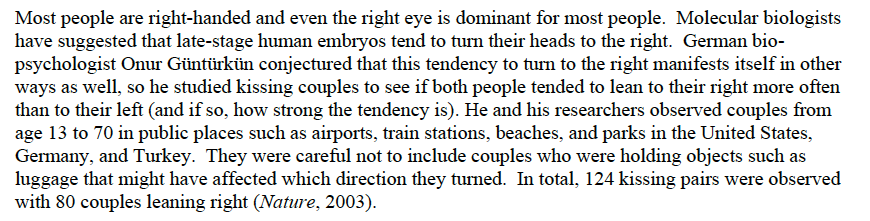
\includegraphics[width=11.5cm,height=5.3 cm]{KissingRight_StudyDescription.png}
\end{center}

\end{frame}
%%%%%%%%%%%%%%%%%%%%%%%%%%%%%%%%%%%%%%%%%%%%%%%

%%%%%%%%%%%%%%%%%%%%%%%%%%%%%%%%%%%%%%%%%%%%%%%%%%%%%%%%%%%%
\begin{frame}[fragile]
%%%%%%%%%%%%%%%%%%%%%%%%%%%%%%%%%%%%%%%%%%%%%%%%%%%%%%%%%%%%
\frametitle{You and your boss !}


\begin{center}

\includegraphics[width=5.5cm,height=5.3 cm]{boss_cartoon.jpg}
\end{center}

\end{frame}
%%%%%%%%%%%%%%%%%%%%%%%%%%%%%%%%%%%%%%%%%%%%%%%


%%%%%%%%%%%%%%%%%%%%%%%%%%%%%%%%%%%%%%%%%%%%%%%%%%%%%%%%%%%%
\begin{frame}[fragile]
%%%%%%%%%%%%%%%%%%%%%%%%%%%%%%%%%%%%%%%%%%%%%%%%%%%%%%%%%%%%

\begin{itemize}
\item \textbf{Boss}: Give me the value of $p$, the actual proportion of people leaning right while kissing !! \pause

\item \textbf{You}: I don't know Sir. But seems like it would be around $\hat{p}=\frac{80}{124} = 0.64$. I know this because

$$ \hat{p} = \frac{1}{124} \sum_{i=1}^{124} X_{i}  $$ \pause

where

$$ X_{i} \sim Ber (p)  $$ \pause

$$  E(X_i) = p \; \forall i \hspace{1 cm} E \left (\frac{1}{124} \sum_{i=1}^{124} X_{i} \right ) = p $$ \pause

implying

$$  E(\hat{p}) = p $$ \pause

\end{itemize}

\end{frame}
%%%%%%%%%%%%%%%%%%%%%%%%%%%%%%%%%%%%%%%%%%%%%%%

%%%%%%%%%%%%%%%%%%%%%%%%%%%%%%%%%%%%%%%%%%%%%%%%%%%%%%%%%%%%
\begin{frame}[fragile]
%%%%%%%%%%%%%%%%%%%%%%%%%%%%%%%%%%%%%%%%%%%%%%%%%%%%%%%%%%%%

\begin{itemize}
\item \textbf{Boss}: Thats not good enough, can you give me an interval where you are absolutely confident will contain the actual $p$?  \pause

\item \textbf{You}: I am $100 \%$ confident that the interval $[0,1]$ will contain the actual $p$ Sir. \pause

\item \textbf{Boss}: Seriously!! Thats all you got from the study?  \pause

\item \textbf{You}: No Sir, I am not $100 \%$ confident, but I am more or less $95\%$ confident that $p$ lies in the intrval $\left [0.556, 0.723 \right] $ Sir. \pause

\item \textbf{Boss} : How on earth did you get that interval?  \pause

\end{itemize}

\end{frame}
%%%%%%%%%%%%%%%%%%%%%%%%%%%%%%%%%%%%%%%%%%%%%%%%%%%%%%%%%%%%%


%%%%%%%%%%%%%%%%%%%%%%%%%%%%%%%%%%%%%%%%%%%%%%%%%%%%%%%%%%%%
\begin{frame}[fragile]
%%%%%%%%%%%%%%%%%%%%%%%%%%%%%%%%%%%%%%%%%%%%%%%%%%%%%%%%%%%%

Well, since $n$ is moderately large, I assumed

$$ \hat{p} \sim N \left ( p, \frac{p(1-p)}{n} \right)  $$ \pause

That meant

$$ \sqrt{n} \frac{\hat{p} - p}{\sqrt{p(1-p)}} \sim N(0,1)  $$ \pause

So, I can write this as $Z = \sqrt{n} \frac{\hat{p} - p}{\sqrt{p(1-p)}}$. From normal table I know

$$ Pr [ - 1.96 < Z < 1.96] = 0.95 $$ \pause

$$ Pr [ - 1.96 < \sqrt{n} \frac{\hat{p} - p}{\sqrt{p(1-p)}}  < 1.96] = 0.95 $$ \pause

$$ Pr [ \hat{p} - 1.96 \frac{\sqrt{p(1-p)}}{\sqrt{n}} < p < \hat{p} + 1.96 \frac{\sqrt{p(1-p)}}{\sqrt{n}}  ] = 0.95 $$ \pause

\end{frame}
%%%%%%%%%%%%%%%%%%%%%%%%%%%%%%%%%%%%%%%%%%%%%%%%%%%%%%%%%%%%%

%%%%%%%%%%%%%%%%%%%%%%%%%%%%%%%%%%%%%%%%%%%%%%%%%%%%%%%%%%%%
\begin{frame}[fragile]
%%%%%%%%%%%%%%%%%%%%%%%%%%%%%%%%%%%%%%%%%%%%%%%%%%%%%%%%%%%%

\begin{itemize}

\item \textbf{Boss}: So? How do you calculate the left and right sides? You don't know $p$ ? \pause

\item \textbf{You}: Well I cheated a bit Sir. and wrote


$$ Pr \left [ \hat{p} - 1.96 \frac{\sqrt{\hat{p}(1-\hat{p})}}{\sqrt{n}} < p < \hat{p} + 1.96 \frac{\sqrt{\hat{p}(1-\hat{p})}}{\sqrt{n}}  \right ] \approx 0.95 $$ \pause

Then I calculate the right and left side by putting $\hat{p}=.64$ and I get the interval $ \left [ 0.56, 0.72 \right]$. \pause

\item \textbf{Boss}: So I get

$$ Pr [ 0.56 < p < 0.72 ] \approx 0.95 $$ \pause

\item \textbf{You}: Well no Sir, that statement is not right!.

\end{itemize}

\end{frame}
%%%%%%%%%%%%%%%%%%%%%%%%%%%%%%%%%%%%%%%%%%%%%%%%%%%%%%%%%%%%%

%%%%%%%%%%%%%%%%%%%%%%%%%%%%%%%%%%%%%%%%%%%%%%%%%%%%%%%%%%%%
\begin{frame}[fragile]
%%%%%%%%%%%%%%%%%%%%%%%%%%%%%%%%%%%%%%%%%%%%%%%%%%%%%%%%%%%%

\begin{itemize}

\item \textbf{Boss}: WTH, isn't that what you just did?  \pause

\item \textbf{You}: Well let me explain Sir. I said with $95 \%$ chance, the true $p$ will lie in the interval

$$ p \in \left [\hat{p} - 1.96 \frac{\sqrt{\hat{p}(1-\hat{p})}}{\sqrt{n}},  \hat{p} + 1.96 \frac{\sqrt{\hat{p}(1-\hat{p})}}{\sqrt{n}} \right] $$ \pause

and I have one such realization of this random interval from experiment and that is $\left [ 0.56, 0.72 \right]$. Thats why I am saying there is a $95 \%$ chance this interval could contain $p$.  \pause

\item \textbf{Boss}: Okay whatever! These numbers $ 0.56 $ and $ 0.72 $ do not look pretty. How about the interval $ \left [ 0.6, 0.7 \right]$. Can you also say you are $ 90\% $ or something confident of that?  \pause

\end{itemize}

\end{frame}
%%%%%%%%%%%%%%%%%%%%%%%%%%%%%%%%%%%%%%%%%%%%%%%%%%%%%%%%%%%%%

%%%%%%%%%%%%%%%%%%%%%%%%%%%%%%%%%%%%%%%%%%%%%%%%%%%%%%%%%%%%
\begin{frame}[fragile]
%%%%%%%%%%%%%%%%%%%%%%%%%%%%%%%%%%%%%%%%%%%%%%%%%%%%%%%%%%%%

\begin{itemize}

\item \textbf{You}: Let me check. \pause

Given that $\hat{p}=0.64$, and you want to find the confidence for $p \in \left [ 0.60, 0.70 \right]$, we can try to look at the probability

$$ Pr \left [ \hat{p} - 0.04 < p < \hat{p} + 0.06 \right ] $$ \pause

or

$$ Pr \left [ -0.06 < \hat{p} - p < 0.04 \right ] $$  \pause

$$ Pr \left [ -\sqrt{n} \frac{0.06}{\sqrt{p(1-p)}} < \sqrt{n}\frac{(\hat{p} - p)}{\sqrt{p(1-p)}} < \sqrt{n} \frac{0.04}{\sqrt{p(1-p)}} \right ] $$ \pause

Then I cheat again

\end{itemize}

\end{frame}
%%%%%%%%%%%%%%%%%%%%%%%%%%%%%%%%%%%%%%%%%%%%%%%%%%%%%%%%%%%%%

%%%%%%%%%%%%%%%%%%%%%%%%%%%%%%%%%%%%%%%%%%%%%%%%%%%%%%%%%%%%
\begin{frame}[fragile]
%%%%%%%%%%%%%%%%%%%%%%%%%%%%%%%%%%%%%%%%%%%%%%%%%%%%%%%%%%%%

$$ Pr \left [ -\sqrt{n}\frac{0.06}{\sqrt{\hat{p}(1-\hat{p})}} < Z < \sqrt{n} \frac{0.04}{\sqrt{\hat{p}(1-\hat{p})}} \right ] $$

$$ \textcolor{red}{Pr \left [ -1.414214 < Z < 0.942809 \right ] \approx 0.7484612} $$

So, I am $75 \%$ confident that the actual $p$ lies in the interval

$$ p \in [\hat{p} - 0.04, \hat{p} + 0.06] := [0.60, 0.70] $$ \pause

\begin{itemize}
\item \textbf{Boss}: What? I just approximate to nearest first decimal, and now you reduced your confidence by $20 \%$? Are you serious? \pause

\item \textbf{You}: Not my fault Sir, its the distribution to blame. \pause
\end{itemize}

\end{frame}
%%%%%%%%%%%%%%%%%%%%%%%%%%%%%%%%%%%%%%%%%%%%%%%%%%%%%%%%%%%%%

%%%%%%%%%%%%%%%%%%%%%%%%%%%%%%%%%%%%%%%%%%%%%%%%%%%%%%%%%%%%
\begin{frame}[fragile]
%%%%%%%%%%%%%%%%%%%%%%%%%%%%%%%%%%%%%%%%%%%%%%%%%%%%%%%%%%%%

\begin{itemize}

\item \textbf{Boss}: Okay let me just report the $95 \%$ interval then, what was that $(0.56, 0.72)$ right?  \pause

\item \textbf{You}: Well kind of. \pause

\item \textbf{Boss}: What do you mean kind of? \pause

\item \textbf{You}: Well I cheated in the middle and used replace $p$ by $\hat{p}$ and said essentially

$$ \sqrt{n} \frac{\hat{p} - p}{\sqrt{\hat{p}(1-\hat{p})}} \approx N(0,1) $$

instead of

$$ \sqrt{n} \frac{\hat{p} - p}{\sqrt{p(1-p)}} \sim N(0,1) $$

which was the correct statement.

\item \textbf{Boss}: I can't write \textit{kind of} in my report. Can't you give me a more exact interval?

\end{itemize}

\end{frame}
%%%%%%%%%%%%%%%%%%%%%%%%%%%%%%%%%%%%%%%%%%%%%%%%%%%%%%%%%%%%%

%%%%%%%%%%%%%%%%%%%%%%%%%%%%%%%%%%%%%%%%%%%%%%%%%%%%%%%%%%%%
\begin{frame}[fragile]
%%%%%%%%%%%%%%%%%%%%%%%%%%%%%%%%%%%%%%%%%%%%%%%%%%%%%%%%%%%%

\begin{itemize}

\item \textbf{You}: I can say exactly that

$$ \sqrt{n} \frac{\hat{p} - p}{\sqrt{\hat{p}(1-\hat{p})}} \sim t_{n-1} $$

where $t_{n-1}$ is another distribution (called \textit{Student's t} distribution).

\item \textbf{Boss}: Where did you come up with that distribution from?

\item \textbf{You}: Okay let me explain.

\end{itemize}

\end{frame}
%%%%%%%%%%%%%%%%%%%%%%%%%%%%%%%%%%%%%%%%%%%%%%%%%%%%%%%%%%%%%

%%%%%%%%%%%%%%%%%%%%%%%%%%%%%%%%%%%%%%%%%%%%%%%%%%%%%%%%%%%%
\begin{frame}{How is the $T-$distribution Related to Estimation?}
%%%%%%%%%%%%%%%%%%%%%%%%%%%%%%%%%%%%%%%%%%%%%%%%%%%%%%%%%%%%

Let $X_1,X_2,\ldots,X_n$ be a random sample
from a $N(\mu,\sigma^2)$ popn.
\medskip

We know that $\displaystyle Z=\frac{\bar{X}-\mu}{\sigma/\sqrt{n}}\sim N(0,1).$ \pause
\medskip

But what if $\sigma^2$ is not known? \pause
Use $s\approx\sigma$ to estimate it.
\bigskip

Consider
\begin{align*}
T &= \frac{\bar{X}-\mu}{s/\sqrt{n}}
= \frac{\bar{X}-\mu}{\sigma/\sqrt{n}} \cdot \frac{\sigma}{s}
= Z \frac{\sigma}{s} \quad
 (\mbox{where\ } Z\sim N(0,1) )
\sim t_{(n-1)}
\end{align*}
\pause

\end{frame}
%%%%%%%%%%%%%%%%%%%%%%%%%%%%%%%%%%%%%%%%%%%%%%%%%%%%%%%%%%%%

%%%%%%%%%%%%%%%%%%%%%%%%%%%%%%%%%%%%%%%%%%%%%%%%%%%%%%%%%%%%
\begin{frame}{$T$ distribution look.....}
%%%%%%%%%%%%%%%%%%%%%%%%%%%%%%%%%%%%%%%%%%%%%%%%%%%%%%%%%%%%

\begin{center}
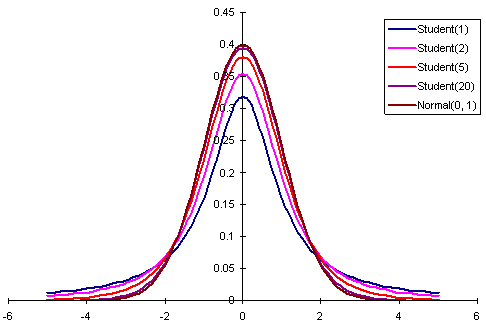
\includegraphics[width=11.5cm,height=5.3 cm]{T-distribution-2.png}
\end{center}

\end{frame}
%%%%%%%%%%%%%%%%%%%%%%%%%%%%%%%%%%%%%%%%%%%%%%%%%%%%%%%%%%%%

%%%%%%%%%%%%%%%%%%%%%%%%%%%%%%%%%%%%%%%%%%%%%%%%%%%%%%%%%%%%
\begin{frame}{How is the $T-$distribution Related to Estimation?}
%%%%%%%%%%%%%%%%%%%%%%%%%%%%%%%%%%%%%%%%%%%%%%%%%%%%%%%%%%%%


$T = \frac{\bar{X}-\mu}{s/\sqrt{n}} \sim t_{(n-1)}$ \pause

\bigskip

So, even when the popn variance $\sigma^2$ is not known, we can
still find probabilities for the sample mean $\bar{X}$ for data from a
normal popn. \pause
\medskip

We just replace $\sigma$ by its estimate $(s)$ in the standardization of
$\bar{X}$ and then look up probabilities from the $t_{(n-1)}$ distribution
instead of the $N(0,1)$ distribution. \pause
\bigskip

The $t_{(n-1)}$ distribution is similar to the $N(0,1),$ but with more
spread (to account for the extra uncertainty in the estimate of $\sigma$.)
\medskip \pause

As sample size increases, $s$ gets closer to $\sigma$ \\
and the $t_{(n-1)}$ distribution gets closer to $N(0,1).$ \pause

\end{frame}
%%%%%%%%%%%%%%%%%%%%%%%%%%%%%%%%%%%%%%%%%%%%%%%%%%%%%%%%%%%%

%%%%%%%%%%%%%%%%%%%%%%%%%%%%%%%%%%%%%%%%%%%%%%%%%%%%%%%%%%%%
\begin{frame}{Connection to the problem here}
%%%%%%%%%%%%%%%%%%%%%%%%%%%%%%%%%%%%%%%%%%%%%%%%%%%%%%%%%%%%

$$ s : = \sqrt{\hat{p} (1 - \hat{p})}  $$

$$ \bar{X} : = \hat{p} $$ \pause

As a result, we can write

$$ \sqrt{n} \frac{\hat{p} - p}{\sqrt{\hat{p}(1-\hat{p})}} \sim t_{n-1} $$ \pause


The t-distribution is nice because it is well-documented, meaning there is a table for $t_{n-1}$ of the probabilities just as there is a table for $N(0,1)$ as you amust be familiar with by now.


\end{frame}
%%%%%%%%%%%%%%%%%%%%%%%%%%%%%%%%%%%%%%%%%%%%%%%%%%%%%%%%%%%%

%%%%%%%%%%%%%%%%%%%%%%%%%%%%%%%%%%%%%%%%%%%%%%%%%%%%%%%%%%%%
\begin{frame}{t distribution}
%%%%%%%%%%%%%%%%%%%%%%%%%%%%%%%%%%%%%%%%%%%%%%%%%%%%%%%%%%%%

A random variable $T \sim t_{n-1}$ distribution

$$ Pr \left [ -1.979 < T_{(n-1)= 123} < 1.979 \right ] = 0.95 $$ \pause

We know 

$$ Pr \left [ -1.959 < Z < 1.959 \right ] = 0.95  $$ \pause
$$ Pr [ \hat{p} - 1.98 \frac{\sqrt{\hat{p}(1-\hat{p})}}{\sqrt{n}} < p < \hat{p} + 1.98 \frac{\sqrt{\hat{p}(1-\hat{p})}}{\sqrt{n}}  ] = 0.95 $$ \pause
$$ 95 \; \%  \; CI \; for \; p \; (t) : \left [ 0.554, 0.725 \right ] $$ \pause
$$ 95 \; \%  \; CI \; for \; p \; (z) : \left [ 0.56, 0.72 \right ] $$

\end{frame}
%%%%%%%%%%%%%%%%%%%%%%%%%%%%%%%%%%%%%%%%%%%%%%%%%%%%%%%%%%%%

%%%%%%%%%%%%%%%%%%%%%%%%%%%%%%%%%%%%%%%%%%%%%%%%%%%%%%%%%%%%
\begin{frame}{One sided interval}
%%%%%%%%%%%%%%%%%%%%%%%%%%%%%%%%%%%%%%%%%%%%%%%%%%%%%%%%%%%%

\begin{itemize}
\item \textbf{Boss}: I want a confidence interval $[c, 1]$ since I know $p$ is very high. So, give me a $95 \%$ confidence interval such that $p \geq c$ instead of $a \leq p \leq b$.  \pause

\item \textbf{You}:  We know that

$$ Pr \left [ Z > -1.645 \right ] \approx 0.95 $$ \pause

That means if we use the normal approximation

$$ Pr \left [  \sqrt{n} \frac{\hat{p} - p}{\sqrt{\hat{p}(1-\hat{p})}} > -1.645 \right ] \approx 0.95 $$ \pause

$$ Pr \left [ p >  \hat{p} - 1.645 \frac{\sqrt{\hat{p}(1-\hat{p})}}{\sqrt{n}} \right] \approx 0.95 $$ \pause

Then the value of $c$

$$ c: \hat{p} - 1.645 \frac{\sqrt{\hat{p}(1-\hat{p})}}{\sqrt{n}} = 0.569 $$ \pause
\end{itemize}

\end{frame}
%%%%%%%%%%%%%%%%%%%%%%%%%%%%%%%%%%%%%%%%%%%%%%%%%%%%%%%%%%%%

%%%%%%%%%%%%%%%%%%%%%%%%%%%%%%%%%%%%%%%%%%%%%%%%%%%%%%%%%%%%
\begin{frame}{One-sided interval}
%%%%%%%%%%%%%%%%%%%%%%%%%%%%%%%%%%%%%%%%%%%%%%%%%%%%%%%%%%%%

\begin{itemize}
\item \textbf{Boss}: I want a confidence interval $[c, 1]$ since I know $p$ is very high. So, give me a $95 \%$ confidence interval such that $p \geq c$ instead of $a \leq p \leq b$. \pause

\item \textbf{You}:  We know that

$$ Pr \left [ T_{123} > -1.657 \right ] \approx 0.95 $$ \pause

That means if we use the normal approximation

$$ Pr \left [  \sqrt{n} \frac{\hat{p} - p}{\sqrt{\hat{p}(1-\hat{p})}} > -1.657 \right ] \approx 0.95 $$ \pause

$$ Pr \left [ p >  \hat{p} - 1.657 \frac{\sqrt{\hat{p}(1-\hat{p})}}{\sqrt{n}} \right] \approx 0.95 $$ \pause

Then the value of $c$

$$ c: \hat{p} - 1.657 \frac{\sqrt{\hat{p}(1-\hat{p})}}{\sqrt{n}} = 0.5685 $$ \pause
\end{itemize}

\end{frame}
%%%%%%%%%%%%%%%%%%%%%%%%%%%%%%%%%%%%%%%%%%%%%%%%%%%%%%%%%%%%

%%%%%%%%%%%%%%%%%%%%%%%%%%%%%%%%%%%%%%%%%%%%%%%%%%%%%%%%%%%%
\begin{frame}{Hypothesis testing}
%%%%%%%%%%%%%%%%%%%%%%%%%%%%%%%%%%%%%%%%%%%%%%%%%%%%%%%%%%%%

\begin{itemize}
\item \textbf{Boss}: Okay I am reporting that I am $95\%$ confident that $p$ lies in $ \left [0.5685, 1 \right]$.

\item \textbf{You}: Sure.

\item \textbf{Boss}: So we can say now that there is effect of leaning on right with kissing .

\item \textbf{You}: Yes you can. Thats because the $95\%$ CI does not contain $0.5$.

\item \textbf{Boss}: Ohh, how did you work that out?

\end{itemize}

\end{frame}
%%%%%%%%%%%%%%%%%%%%%%%%%%%%%%%%%%%%%%%%%%%%%%%%%%%%%%%%%%%%

%%%%%%%%%%%%%%%%%%%%%%%%%%%%%%%%%%%%%%%%%%%%%%%%%%%%%%%%%%%%
\begin{frame}{Connection: testing and CI}
%%%%%%%%%%%%%%%%%%%%%%%%%%%%%%%%%%%%%%%%%%%%%%%%%%%%%%%%%%%%

If you are testing

$$ H_0 : p = 0.5 \hspace{1 cm}  H_1: p > 0.5 $$ \pause

then if you want to test and reject the null when p-value $< 0.05$, then you just check if the null hypothesis $p$, which is $0.5$, lies in the one sided confidence interval $[c,1]$.  \pause

Does the confidence interval $ [0.5685, 1] $ contains $0.5$?  Ans: NO
So, we reject the null.\pause

If you test

$$ H_0 : p = 0.5 \hspace{1 cm}  H_1: p \neq 0.5 $$ \pause

Then check if the 2-sided $95 \%$ interval $ [a, b] $ contains $0.5$, here we observe that $\left [ 0.554, 0.725 \right ] $ does not contain $0.5$. so, again we reject the null.  \pause

For detailed explanation of this, check Canvas. \pause

\end{frame}
%%%%%%%%%%%%%%%%%%%%%%%%%%%%%%%%%%%%%%%%%%%%%%%%%%%%%%%%%%%%

%%%%%%%%%%%%%%%%%%%%%%%%%%%%%%%%%%%%%%%%%%%%%%%%%%%%%%%%%%%%
\begin{frame}{Confidence intervals}
%%%%%%%%%%%%%%%%%%%%%%%%%%%%%%%%%%%%%%%%%%%%%%%%%%%%%%%%%%%%

\begin{itemize}

\item \textbf{Boss}: Great! So, I am going to write \textit{I am pretty sure that there is a tendency of people leaning to the right while kissing and I am $95 \%$ confident that this probability lies in $ [ 0.5685, 1] $ if I assume the interval to be one-sided and in $ [ 0.554, 0.725 ] $ if the interval is two-sided}. How does that sound? \pause

\item \textbf{You}: Sounds very good Sir. But you should mention $95 \%$ confident under assumption of normality/ t-distribution.  \pause

\item \textbf{Boss}: What other alternative did we have? Can the conclusion change if we drop the assumption? \pause

\item \textbf{You}: The alternative is called Bootstrap confidence interval and the conclusion may very well change sir, especially for non-normal distributed random variables with small sample size.  \pause

\item \textbf{Boss}: Why don't you calculate this Bootstrap CI and check? \pause

\end{itemize}

\end{frame}
%%%%%%%%%%%%%%%%%%%%%%%%%%%%%%%%%%%%%%%%%%%%%%%%%%%%%%%%%%%%

%%%%%%%%%%%%%%%%%%%%%%%%%%%%%%%%%%%%%%%%%%%%%%%%%%%%%%%%%%%%
\begin{frame}{General idea: Bootstrapping/ Resampling}
%%%%%%%%%%%%%%%%%%%%%%%%%%%%%%%%%%%%%%%%%%%%%%%%%%%%%%%%%%%%

Let $X_1, X_2, \cdots, X_{n}$ be data corresponding to $n$ samples coming from a distribution $F$, where $F$ is not unknown and there is no reason to assume normality.\pause \newline

Suppose we want to find the sampling distribution of $\bar{X}$.  \pause \newline

We know if $n$ is large, then this sampling distribution is normal, and

$$ \bar{X} \sim N(\mu, \frac{\sigma^2}{n})  \hspace{0.5 cm} for \;\; large \;\; n$$

where $\mu$ and $\sigma$ are the population mean and population standard deviation under the population distribution or model $F$ (again may not be normal). \pause \newline

If $n$ is not so large though, normality is not a good assumption for sampling distribution.

\end{frame}
%%%%%%%%%%%%%%%%%%%%%%%%%%%%%%%%%%%%%%%%%%%%%%%%%%%%%%%%%%%%

%%%%%%%%%%%%%%%%%%%%%%%%%%%%%%%%%%%%%%%%%%%%%%%%%%%%%%%%%%%%
\begin{frame}
%%%%%%%%%%%%%%%%%%%%%%%%%%%%%%%%%%%%%%%%%%%%%%%%%%%%%%%%%%%%

\frametitle{Bootstrapping}

This is a special technique of resampling. \pause This is useful:

\begin{itemize}
\item When the theoretical distribution of a statistic of interest is complicated or unknown. \pause
\item When the sample size is insufficient for straightforward statistical inference. \pause
\end{itemize}

\end{frame}
%%%%%%%%%%%%%%%%%%%%%%%%%%%%%%%%%%%%%%%%%%%%%%%%%%%%%%%%%%%%

%%%%%%%%%%%%%%%%%%%%%%%%%%%%%%%%%%%%%%%%%%%%%%%%%%%%%%%%%%%%
\begin{frame}
%%%%%%%%%%%%%%%%%%%%%%%%%%%%%%%%%%%%%%%%%%%%%%%%%%%%%%%%%%%%

\frametitle{Bootstrapping to find CI}

You want to find the CI for $\mu$, the population mean. \pause
\begin{itemize}
\item Take 1000 resamples and evaluate the sample means for them. \pause
\item Those 1000 values of the means give you the {\it Bootstrap distribution}. \pause
\item Find the 2.5th and the 97.5th quantile from that distribution. \pause
\item In other words, sort those values and find 25th and 975th values. Those will give you the CI for the mean. \pause
\end{itemize}

You can use this technique for any parameter of interest!

\end{frame}
%%%%%%%%%%%%%%%%%%%%%%%%%%%%%%%%%%%%%%%%%%%%%%%%%%%%%%%%%%%%


%%%%%%%%%%%%%%%%%%%%%%%%%%%%%%%%%%%%%%%%%%%%%%%%%%%%%%%%%%%%
\begin{frame}[fragile]
%%%%%%%%%%%%%%%%%%%%%%%%%%%%%%%%%%%%%%%%%%%%%%%%%%%%%%%%%%%%

\frametitle{Bootstrapping to find p-value}

You want to find the p-value for a test involving test statistic $T$, say. Suppose you are interested in one-sided alternative (greater than). \pause
\begin{itemize}
\item For the original sample, evaluate $T$. \pause
\item Take $1000$ resamples and evaluate the test statistics ($T$) for them. \pause
\item Those $1000$ values of the means give you the {\it Bootstrap distribution} for $T$. \pause
\item Find how many of them are more extreme than $T$ from the original sample. \pause
\item The proportion gives you the estimated p-value. \pause
\item For CI, find the region that contains $95 \%$ of the $T$ in the Bootstrap samples (for 2-sided the region between the $2.5$ th quantile and $97.5$ th quantile of the Bootstrap $T$ samples, for 1-sided the region beyond $5$ th quantile)
\end{itemize}

You can use this technique to test your hypothesis or build confidence interval if you do not have an idea about the general population distribution.

\end{frame}
%%%%%%%%%%%%%%%%%%%%%%%%%%%%%%%%%%%%%%%%%%%%%%%%%%%%%%%%%%%%

%%%%%%%%%%%%%%%%%%%%%%%%%%%%%%%%%%%%%%%%%%%%%%%%%%%%%%%%%%%%
\begin{frame}[fragile]
%%%%%%%%%%%%%%%%%%%%%%%%%%%%%%%%%%%%%%%%%%%%%%%%%%%%%%%%%%%%



\begin{knitrout}\small
\definecolor{shadecolor}{rgb}{1, 1, 1}\color{fgcolor}\begin{kframe}
\begin{alltt}
\hlstd{obs.samp} \hlkwb{<-} \hlkwd{c}\hlstd{(}\hlkwd{rep}\hlstd{(}\hlnum{1}\hlstd{,}\hlnum{80}\hlstd{),} \hlkwd{rep}\hlstd{(}\hlnum{0}\hlstd{,} \hlnum{44}\hlstd{));}
\hlstd{bootstrap_counts} \hlkwb{<-} \hlkwd{replicate}\hlstd{(}\hlnum{1000}\hlstd{,} \hlkwd{sum}\hlstd{(}\hlkwd{sample}\hlstd{(obs.samp,} \hlkwc{replace}\hlstd{=}\hlnum{TRUE}\hlstd{)))}
\hlkwd{summary}\hlstd{(bootstrap_counts)}
\end{alltt}
\begin{verbatim}
   Min. 1st Qu.  Median    Mean 3rd Qu.    Max. 
   65.0    77.0    80.0    80.2    84.0    95.0 
\end{verbatim}
\begin{alltt}
\hlstd{bootstrap_prop} \hlkwb{<-} \hlstd{bootstrap_counts}\hlopt{/}\hlnum{124}\hlstd{;}
\hlcom{## 2-sided}

\hlkwd{quantile}\hlstd{(bootstrap_prop,} \hlnum{0.025}\hlstd{)}
\end{alltt}
\begin{verbatim}
  2.5% 
0.5645 
\end{verbatim}
\begin{alltt}
\hlkwd{quantile}\hlstd{(bootstrap_prop,} \hlnum{0.975}\hlstd{)}
\end{alltt}
\begin{verbatim}
 97.5% 
0.7258 
\end{verbatim}
\begin{alltt}
\hlcom{## 1-sided}
\hlkwd{quantile}\hlstd{(bootstrap_prop,} \hlnum{0.05}\hlstd{)}
\end{alltt}
\begin{verbatim}
    5% 
0.5806 
\end{verbatim}
\end{kframe}
\end{knitrout}

\end{frame}
%%%%%%%%%%%%%%%%%%%%%%%%%%%%%%%%%%%%%%%%%%%%%%%%%%%%%%%%%%%%

%%%%%%%%%%%%%%%%%%%%%%%%%%%%%%%%%%%%%%%%%%%%%%%%%%%%%%%%%%%%
\begin{frame}
%%%%%%%%%%%%%%%%%%%%%%%%%%%%%%%%%%%%%%%%%%%%%%%%%%%%%%%%%%%%

\begin{itemize}
\item \textbf{You}: Sir, the Bootstap CIs (both 2-sided and 1-sided ) are very close to the normal or t-distribution CIs.  \pause

\item \textbf{Boss}: Okay, here is the final report then: \textit{We find strong evidence that there is indeed a tendency to lean to the right while kissing ($95 \%$ 2-sided CI under normality: $ [ 0.554, 0.725 ] $, Bootstrap CI: $[0.564, 0.725]$  and $95 \%$ 1-sided CI under normality: $ [ 0.5685, 1] $, Bootstrap CI: $[0.5806, 1]$)}. \pause

\item \textbf{You}: That sounds perfect now! \pause

\item \textbf{Boss}: Okay let me submit that then. Thanks. \pause

\item To be continued....

\end{itemize}

\end{frame}
%%%%%%%%%%%%%%%%%%%%%%%%%%%%%%%%%%%%%%%%%%%%%%%%%%%%%%%%%%%%

%%%%%%%%%%%%%%%%%%%%%%%%%%%%%%%%%%%%%%%%%%%%%%%%%%%%%%%%%%%%
\begin{frame}
%%%%%%%%%%%%%%%%%%%%%%%%%%%%%%%%%%%%%%%%%%%%%%%%%%%%%%%%%%%%

Suppose we want to test

$$ H_{0}: p=0.5 \; \; H_{1}: p = 0.8 $$ \pause

In this case, both the hypothesis are \textit{point} hypothesis. \pause

When we encounter such hypothesis? Case: Another researcher has claimed the probability of leaning to the right while kissing is $80 \%$, you want to test this claim.

How do we test such a hypothesis? \pause

We define 2 types of errors. \pause

\end{frame}
%%%%%%%%%%%%%%%%%%%%%%%%%%%%%%%%%%%%%%%%%%%%%%%%%%%%%%%%%%%%

%%%%%%%%%%%%%%%%%%%%%%%%%%%%%%%%%%%%%%%%%%%%%%%%%%%%%%%%%%%%
\begin{frame}
%%%%%%%%%%%%%%%%%%%%%%%%%%%%%%%%%%%%%%%%%%%%%%%%%%%%%%%%%%%%

\begin{tabular}{ c | c  | c }
& $H_0$ is true & $H_a$ is true\\
\hline
Reject $H_0$ & Type I error & Correct decision \\
& $\alpha$ & $1 - \beta = \pi$ \\
\hline
Not reject $H_0$ & Correct decision & Type II error \\
& $1-\alpha$ & $\beta$ \\
\end{tabular}

\begin{itemize}
\item $\alpha = P(\text{Type I Error}) = P(\text{Reject } H_0|H_0 \text{ is true}) = \text{Significance level} $
\item $\beta = P(\text{Type II Error}) = P(\text{Not reject } H_0|H_a \text{ is true})$
\vspace{5mm}
\item We also define \textbf{power} as
\begin{align*}
\pi &= 1 - \beta \\
&= P(\text{Reject } H_0|H_a \text{ is true}) \\
&= \text{Ability to Detect the Alternative Hypothesis}
\end{align*}
\end{itemize}

\end{frame}
%%%%%%%%%%%%%%%%%%%%%%%%%%%%%%%%%%%%%%%%%%%%%%%%%%%%%%%%%%%%

%%%%%%%%%%%%%%%%%%%%%%%%%%%%%%%%%%%%%%%%%%%%%%%%%%%%%%%%%%%%
\begin{frame}
%%%%%%%%%%%%%%%%%%%%%%%%%%%%%%%%%%%%%%%%%%%%%%%%%%%%%%%%%%%%

$$ \alpha = Pr (\text{Type I Error}) = Pr (\text{Reject } H_0|H_0 \text{ is true}) $$

$$ \alpha = Pr (\text{Reject } H_0|p=0.5) $$

Assume we reject $H_0$ if p-value is $< 0.05$, this means if true $p$  under null hypothesis $H_0$ does not lie in the $95 \%$ confidence interval,

put $\hat{p}=0.64$, $p=0.5$,

$$ Pr \left[ p - 1.96 \frac{\sqrt{p(1-p)}}{\sqrt{n}} < \hat{p} < p + 1.96 \frac{\sqrt{p(1-p)}}{\sqrt{n}} \right] = [0.552, 0.728] $$

$p=0.5$ does not belong in this

\end{frame}
%%%%%%%%%%%%%%%%%%%%%%%%%%%%%%%%%%%%%%%%%%%%%%%%%%%%%%%%%%%%















\end{document}
